\documentclass{article}
\usepackage{graphicx}
%permite ecribir acentos directamente
\usepackage[utf8]{inputenc}
% Esto es para que el LÁTEX sepa que el texto está en español, se agrega el ingles para el paquete de gráfico de circuitos:
\usepackage[spanish]{babel}
\usepackage{geometry}
 \geometry{a4paper,total={170mm,257mm},left=15mm,right=15mm,top=20mm,}
\usepackage{hyperref} 
\usepackage{textcomp}

\usepackage{tikz}
\usetikzlibrary{shapes,arrows}

\begin{document}
\begin{titlepage}
 \centering
	
\includegraphics[scale=0.80]{imagenes/LOGO.jpg} \par
 	\vspace{1cm}
 	{\scshape\LARGE Universidad Tecnológica Nacional \par}
 	{\scshape\large Facultad Regional de Córdoba \par}
 	\vspace{1cm}
	{\bfseries \Large Trabajo Práctico $N^{\circ} 1$\par}
	{\bfseries \Large Cálculo de confiabilidad de sistemas electrónicos \par}
 	\vspace{1.5cm}

	\begin{tabular}{ll}
		Navarro, Facundo 	&	63809 	\\
		Veron, Misael	 	&	62628
	\end{tabular}
	
	\vspace{1cm}
	Curso: 5r2 \\
 	\vfill
	{\bfseries \Large Cátedra: Tecnología Electrónica \par}

	\vspace{1.5cm}
	Docentes: \par
	Ing. Centeno, Carlos \par
	Ing. Gonzalez Dondo, Diego \par

 	\vfill
	{\large \today\par}
\end{titlepage}

%##################################### INDICE  #####################################################

\tableofcontents
\clearpage

%##################################### INDICE  #####################################################

\section{Introducción}
En términos de la teoría de administración de recursos, la estadística tiene un papel fundamental, los modelos probabilisticos cuando son aplicados a grandes muestras tienden a "suavizar" las variaciones individuales por lo que el resultado final es lo suficientemente simple y preciso para el análisis de diseño.
En el diseño de cualquier circuito electrónico se debería realizar un previo cálculo de confiabilidad, ya que de esta manera se pone en evidencia las debilidades y fortalezas del mismo. En el siguiente informe se realizará el análisis sobre un circuito utilizando las normas de dos handbook militares, el  HDBK-MIL-217 y el HDBK-MIL-338B, teniendo la ventaja que no se requiere tener el dispositivo construido, permitiendo un análisis preventivo

\section{Circuito a analizar}
Se eligió el shield de relés de Arduino, el cual es controlado por un microcontrolador de la marca PIC, el modelo PIC16F886, el conjunto del PIC con el shield se utilizará para el control autónomo de la luminaria de una vivienda, el sistema se encuentra fijo, sin ser sometido a ningún tipo de vibración, en un ambiente estable y expuesto a una temperatura de entre $24^{\circ}$C y $30^{\circ}$C, a continuación se presenta el esquemático:
\begin{figure}[h]
 \begin{center}
	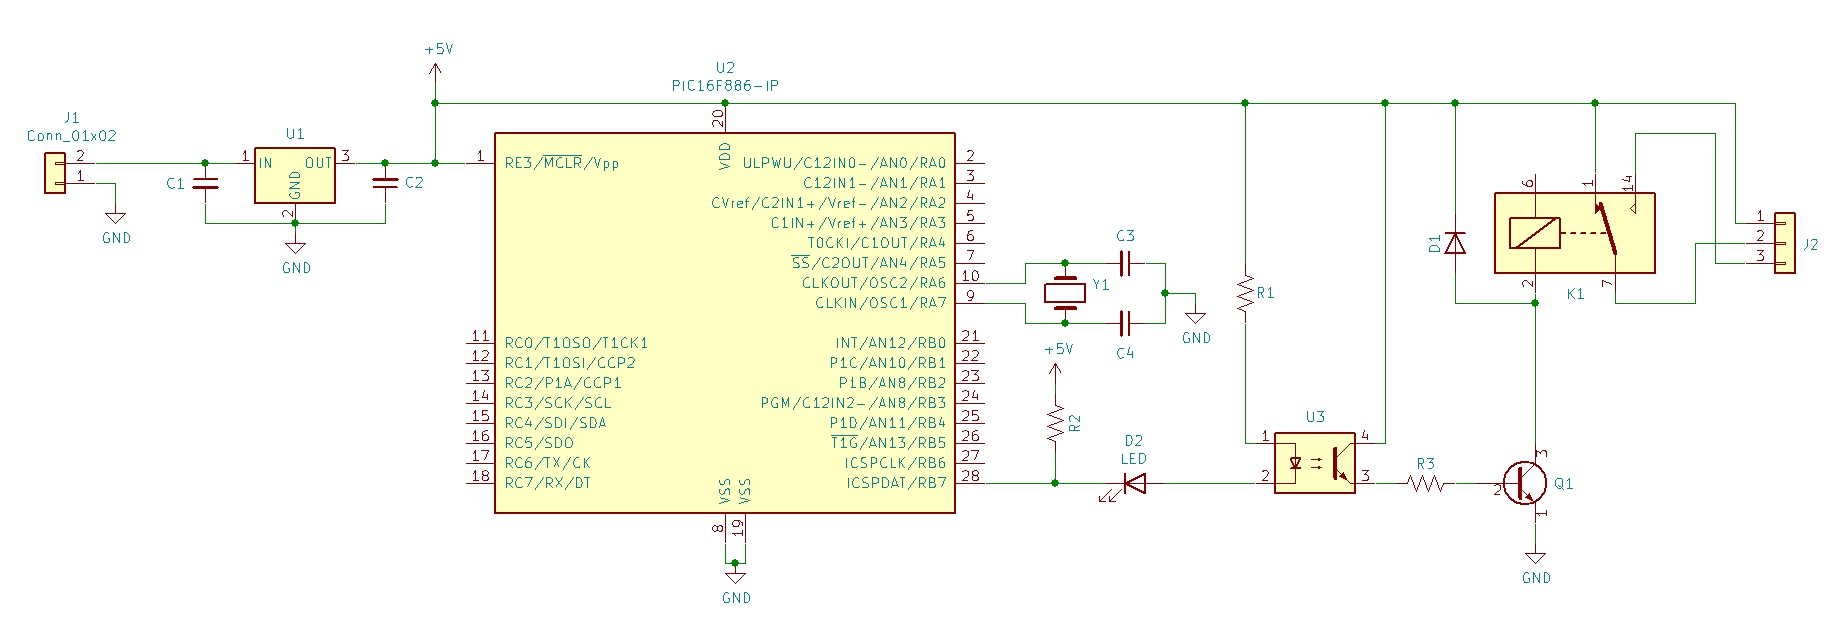
\includegraphics[width=\textwidth]{imagenes/fig1.jpg} 
	\caption{Circuito a analizar}\label{fig:fig1}
 \end{center}
\end{figure}
%

\end{document}